\chapter{Arhitektura i dizajn sustava}

		\section{Baza podataka}
			
		Za našu platformu koristit ćemo relacijsku bazu podataka. Objekt takve baze je relacija, odnosno tablica koja je definirana svojim imenom i skupom atributa. Atributi unutar jednog entiteta mogu poprimiti funkciju primarnog ili stranog ključa.
Baza podataka ove aplikacije sastoji se od 3 entiteta:
		
			\subsection{Opis tablica}
			
\textbf{\textit{login}}\\
\begin{samepage}
Ovaj entitet sastoji se od jednog atributa - atributa username. To je ujedno i primarni ključ entiteta i predstavlja jedinstveni identifikator korisnika - korisničko ime.
\end{samepage}
				
				
				\begin{longtblr}[
					label=none,
					entry=none
					]{
						width = \textwidth,
						colspec={|X[6,l]|X[6, l]|X[20, l]|}, 
						rowhead = 1,
					} %definicija širine tablice, širine stupaca, poravnanje i broja redaka naslova tablice
					\hline \SetCell[c=3]{c}{\textbf{login}}	 \\ \hline[3pt]
					\SetCell{LightGreen}username & VARCHAR	&  	jedinstveni identifikator korisnika 	\\ \hline
				\end{longtblr}

    \eject
\noindent \textbf{\textit{profile}}\\
\begin{samepage}
Ovaj entitet sadrži osnovne informacije o korisničkom profilu i  sastoji se od sljedećih atributa: email (email adresa), username (korisničko ime), name (ime), surname (prezime) i age (dob). Email i username su primarni ključevi entiteta \textbf{profile}, a username ujedno i strani ključ koji povezuje \textbf{profile} i \textbf{login}.
\end{samepage}

    				\begin{longtblr}[
					label=none,
					entry=none
					]{
						width = \textwidth,
						colspec={|X[6,l]|X[6, l]|X[20, l]|}, 
						rowhead = 1,
					} %definicija širine tablice, širine stupaca, poravnanje i broja redaka naslova tablice
     
					\hline \SetCell[c=3]{c}{\textbf{profile}}	 \\ \hline[3pt]
					\SetCell{LightGreen}email & VARCHAR	&  	e-mail adresa korisnika 	\\ \hline
     				\SetCell{LightGreen}username & VARCHAR	&  	jedinstveni identifikator korisnika	\\ \hline
          			\SetCell{} name & VARCHAR	&  ime korisnika 	\\ \hline
               			\SetCell{} surname & VARCHAR	&  	prezime korisnika 	\\ \hline
                    \SetCell{} age & INT	&  	dob korisnika 	\\ \hline
                    
				\end{longtblr}

    
\noindent \textbf{\textit{recipe}}\\
\begin{samepage}
Ovaj entitet opisuje recept postavljen na platformu od strane registriranog korisnika. Primarni je ključ recipeID - ID recepta, a strani ključevi email i username koji povezuju \textbf{recipe} i \textbf{profile}. Ostali atributi su likes - broj oznaka "sviđa mi se" na receptu od strane registriranih korisnika, ingredients - sastojci jela koje recept opisuje, name (ime recepta), instructions (niz uputa pripreme jela opisanog receptom), origin (mjesto podrijetla jela), category (kategorija jela), specialTags - dodatne oznake, URL\_to\_image - URL slike koju korisnik prilaže uz postavljeni recept te URL\_to\_video - URL videa koji korisnik prilaže uz postavljeni recept.
\end{samepage}
    
    				\begin{longtblr}[
					label=none,
					entry=none
					]{
						width = \textwidth,
						colspec={|X[6,l]|X[6, l]|X[20, l]|}, 
						rowhead = 1,
					} %definicija širine tablice, širine stupaca, poravnanje i broja redaka naslova tablice
					\hline \SetCell[c=3]{c}{\textbf{recipe}}	 \\ \hline[3pt]
					\SetCell{LightGreen}recipeID & VARCHAR	&  	jedinstveni identifikator recepta 	\\ \hline
          				\SetCell{LightBlue}email & VARCHAR	&  	e-mail adresa korisnika 	\\ \hline
          			\SetCell{LightBlue}username & VARCHAR	&  	jedinstveni identifikator korisnika 	\\ \hline
               			\SetCell{} likes & INT	&  	broj oznaka "sviđa mi se" recepta 	\\ \hline
                    \SetCell{} ingredients & VARCHAR	&  	popis sastojaka receptnog jela 	\\ \hline
                    \SetCell{} name & VARCHAR	&  	ime recepta 	\\ \hline
                    \SetCell{} instructions & VARCHAR	&  	niz uputa za pripremu jela prema receptu 	\\ \hline
                    \SetCell{} origin & VARCHAR	&  	mjesto podrijetla receptnog jela	\\ \hline
                    \SetCell{} category & VARCHAR	&  	vrsta (kategorija) receptnog jela 	\\ \hline
                    \SetCell{} specialTags & VARCHAR	&  	specijalne dodatne oznake receptnog jela 	\\ \hline
                    \SetCell{} URL\_to\_video & VARCHAR	&  	URL videa priloženog uz recept 	\\ \hline
					\SetCell{} URL\_to\_image & VARCHAR	&  	URL slike priložene uz recept 	\\ \hline
				\end{longtblr}
				
				
			
			\subsection{Dijagram baze podataka}
			
\begin{figure}[h]
			    \centering
			    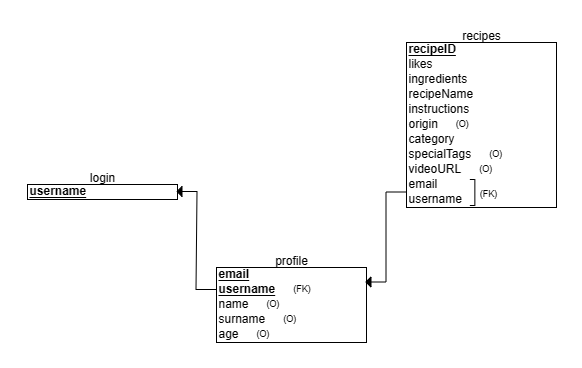
\includegraphics[width=1\linewidth]{slike/ERdiagram.png}
			    \caption{ER dijagram baze podataka}
			    \label{fig:enter-label}
			\end{figure}
			
			\eject
			
			
		\section{Dijagram razreda}
		
			\textit{Potrebno je priložiti dijagram razreda s pripadajućim opisom. Zbog preglednosti je moguće dijagram razlomiti na više njih, ali moraju biti grupirani prema sličnim razinama apstrakcije i srodnim funkcionalnostima.}\\
			
			\textbf{\textit{dio 1. revizije}}\\
			
			\textit{Prilikom prve predaje projekta, potrebno je priložiti potpuno razrađen dijagram razreda vezan uz \textbf{generičku funkcionalnost} sustava. Ostale funkcionalnosti trebaju biti idejno razrađene u dijagramu sa sljedećim komponentama: nazivi razreda, nazivi metoda i vrste pristupa metodama (npr. javni, zaštićeni), nazivi atributa razreda, veze i odnosi između razreda.}\\
			
			\textbf{\textit{dio 2. revizije}}\\			
			
			\textit{Prilikom druge predaje projekta dijagram razreda i opisi moraju odgovarati stvarnom stanju implementacije}
			
			
			
			\eject
		
		\section{Dijagram stanja}
			
			
			\textbf{\textit{dio 2. revizije}}\\
			
			\textit{Potrebno je priložiti dijagram stanja i opisati ga. Dovoljan je jedan dijagram stanja koji prikazuje \textbf{značajan dio funkcionalnosti} sustava. Na primjer, stanja korisničkog sučelja i tijek korištenja neke ključne funkcionalnosti jesu značajan dio sustava, a registracija i prijava nisu. }
			
			
			\eject 
		
		\section{Dijagram aktivnosti}
			
			\textbf{\textit{dio 2. revizije}}\\
			
			 \textit{Potrebno je priložiti dijagram aktivnosti s pripadajućim opisom. Dijagram aktivnosti treba prikazivati značajan dio sustava.}
			
			\eject
		\section{Dijagram komponenti}
		
			\textbf{\textit{dio 2. revizije}}\\
		
			 \textit{Potrebno je priložiti dijagram komponenti s pripadajućim opisom. Dijagram komponenti treba prikazivati strukturu cijele aplikacije.}
